% !TEX root = ./Cours.tex
\documentclass[../€Cours-complet/Cours-complet]{subfiles}

\usetikzlibrary{matrix,arrows,positioning}

\titleorchapter{Proportionnalités et tableaux}{4}

\begin{document}

\maketitleCours

\section{Proportionnalité}

\begin{vocabulaire}[Grandeur]
	Une \textbf{grandeur} est une caractéristique qui se mesure ou se calcule.

	Par exemple le temps, la masse, la taille, le prix...
\end{vocabulaire}

\begin{cours}
	On dit que deux grandeurs sont \textbf{proportionnelles} si on peut obtenir l'une en multipliant l'autre par un nombre fixé. Ce nombre est appelé \textbf{coefficient de proportionnalité}.
\end{cours}

\begin{exemple}
	On va acheter des livres en librairie : chaque livre coûte 10€.

	\begin{itemize}
		\item La première grandeur est \textbf{le nombre de livres}.
		\item La deuxième grandeur est \textbf{le prix des livres}.
	\end{itemize}

	Les deux grandeurs sont donc \textbf{proportionnelles}, car il suffit de multiplier le nombre de livres par 10 pour avoir le prix.
\end{exemple}

\begin{exemple}
	La taille d'une personne n'est pas proportionnelle à son âge : si je mesure 1,50 mètres à 15 ans, je ne ferais pas 6 mètres à 60 ans !
\end{exemple}

\begin{cours}
	Dans un \textbf{tableau de proportionnalité}, les nombres de la première ligne sont proportionnels avec ceux de la deuxième ligne.
\end{cours}

\begin{exemple}
	On mesure la distance parcourue par une voiture en deux heures, en fonction de sa vitesse : \vspace{0.5em}

	\begin{tabular}{|l|c|c|c|c|}
		\hline
		Vitesse            & 20km/h & 50km/h & 40km/h & 120km/h \\ \hline
		Distance parcourue & 40km   & 100km  & 80km   & 240km   \\ \hline
	\end{tabular}

	C'est un tableau de proportionnalité, car on obtient la deuxième ligne en multipliant la première par deux.
\end{exemple}

\section{Quatrième proportionnelle}

\begin{cours}
	Si un tableau de proportionnalité a quatre case, dont une seule vide, alors \textbf{on peut calculer la quatrième valeur}, qu'on appelle alors \textbf{quatrième proportionnelle}.
\end{cours}

\begin{methode}
	Pour trouver une quatrième proportionnelle :
	\begin{itemize}
		\item Une des colonnes du tableau est remplie : on peut donc trouver le \\ \myuline{coefficient de proportionnalité}.
		\item Si la valeur manquante est en bas, on \textbf{multiplie} la case au dessus par le coefficient de proportionnalité.
		\item Si la valeur manquante est en haut, on \textbf{divise} la case en dessous par le coefficient de proportionnalité.
	\end{itemize}
\end{methode}

\begin{exemple}
	On sait que le tableau suivant est proportionnel :

	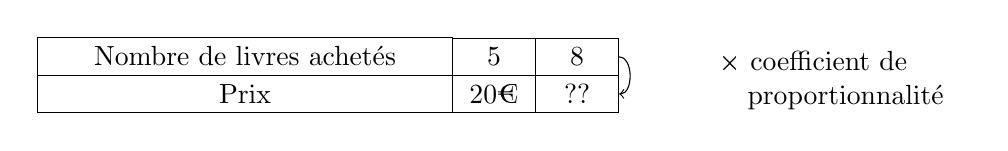
\begin{tikzpicture}
		\matrix (tableau) [
			nodes={rectangle,draw=black,minimum width=3em},
			matrix of nodes,
			row sep=-\pgflinewidth,
			column sep=-\pgflinewidth,
			column 1/.style={
					minimum width=15em,
					nodes={rectangle,draw=black,minimum width=15em}
				}]{
			Nombre de livres achetés & 5   & 8  \\
			Prix                     & 20€ & ?? \\
		};
		\draw[->] (tableau-1-3.east) to [out=0,in=0] (tableau-2-3.east);
		\node[text width=4cm,align=center] at ([xshift=3cm,yshift=-0.3cm] tableau-1-3) {× coefficient de\\ \hspace{2em} proportionnalité};
	\end{tikzpicture}  \\
	Le coefficient de proportionnalité est
	$$ 20 ÷ 5 = 4 $$
	Donc le prix de 8 livres est
	$$ 8 × 4 = 32€ $$
\end{exemple}

\begin{greybox}[frametitle={Remarque}]
	On peut aussi passer d'une colonne à l'autre en multipliant/divisant par un nombre.

	Ce nombre change selon les colonnes.
\end{greybox}

\section{Pourcentages}

\begin{cours}
	Calculer \textbf{x\%} d'une quantité revient à calculer cette quantité multipliée par $\frac{\text{x}}{100}$.
\end{cours}

\begin{exemple}
	On a une réduction de 15\% sur un gâteau qui coûte 10€.

	On paie donc 15\% en moins, c'est-à-dire $\frac{15}{100} × 10 = 1,50€$ de moins.
\end{exemple}

\begin{cours}[Calculer un pourcentage]
	Pour calculer un pourcentage à partir d'une fraction, il faut mettre le \textbf{dénominateur} de la fraction à 100.
\end{cours}

\section{Durées et horaires}

\begin{cours}[Durées]
	\begin{itemize}
		\item Dans une minute, il y a 60 secondes.
		\item Dans une heure, il y a 60 minutes.
		\item Dans une heure, il y a 3600 secondes.
		\item Dans une journée, il y a 24 heures.
		\item Dans une année, il y a 365 jours (sauf pendant une année bissextile).
	\end{itemize} \vspace{1em}

	Toutes ces grandeurs sont \textbf{proportionnelles}.
\end{cours}

\end{document}